\documentclass[11pt,a5paper]{book}
\usepackage[utf8]{inputenc}
\usepackage{amsmath}
\usepackage{amsfonts}
\usepackage{amssymb}
\usepackage{graphicx}
\usepackage[super]{nth}

\title{One Fish, Two Fish}
\author{Marcel Gietzmann-Sanders}
\date{}
\setcounter{tocdepth}{1}
\begin{document}
\maketitle
\tableofcontents
\newpage
\chapter{How to Digest a Brick}

\section{The Whole Point}

Quantitative fisheries science (hereafter referred to just as fisheries modeling) is all about answer the following question:
\newline

\hangafter=0 \hangindent=1cm \noindent How can a fishery bring the maximum long term benefits to society?
\newline

Even in just this question there is a lot to unpack. What's a fishery? What do we mean by maximum? What's does long term mean and how do we quantify benefit? And who is this society? Also what kinds of answers count for the "How" that starts that whole sentence? 
\newline

While no answer to these kinds of questions is going to ever be complete or 100\% right let's at least get a sense of what flavor the answer might be. Let's take each component (shown in \textbf{bold}) in turn.
\newpage

\noindent \rule{\textwidth}{0.5pt} 
\noindent How can a \textbf{fishery} bring the maximum long term benefits to society?
\newline
\rule{\textwidth}{0.5pt} 
\vspace{5pt}

A fishery can be a lot of things. Fishers use all sorts of different kinds of tackle - nets, hooks, trawls, etc. - to catch all manner of sea creatures - fish, turtles, crustaceans, etc. Those creatures live all over the globe, have all sorts of species, populations, and communities, spawn in some areas, forage in others, and so on. Likewise the fishers who catch them operate in all kinds of ways at all kinds of times in all sorts of places. So clearly a fishery can mean a lot of things. It could mean a specific type of tackle used at a certain time of year in a specific place to catch a specific thing, it could mean anyone who tries to take a specific species in a specific area, or it could mean anyone fishing in a specific ecosystem. Yikes! That's not much of a definition. Herein we're going to designate fisheries by the species populations that they affect. This gives us the freedom to either choose to concern ourselves with a single species at a time or deal with ecosystems as a whole - the only difference is how many species we consider. 
\newpage

\noindent \rule{\textwidth}{0.5pt} 
\noindent How can a fishery bring the maximum long term \textbf{benefits} to society?
\newline
\rule{\textwidth}{0.5pt} 
\vspace{5pt}

This one is also ridiculously tricky. Benefits from seafood can be nutritional, cultural, financial, and biological (amongst other things). They can make or break communities, they can be necessary for raising other farmed fish or fertilizing farms. Some fisheries have important medical applications. And all fisheries are subject to the creativity of entrepreneurs - it wasn't so long ago that lobster was prison food. So when quantifying benefit the answer is \textit{absolutely} specific to the fishery in question. As much as folks would like to provide some singular answer, the fact is each fishery has a whole load of different values. \textit{Know your fishery}.
\newpage

\noindent \rule{\textwidth}{0.5pt} 
\noindent How can a fishery bring the maximum \textbf{long term} benefits to society?
\newline
\rule{\textwidth}{0.5pt} 
\vspace{5pt}

Whatever the benefits accrued the hope is that those benefits remain with us over the long term - i.e. that they are sustainable benefits. Fishing a region to death only means that short term benefits rob us from long term sustained (and therefore much larger) benefits. So by long term we mean sustainable. 
\newpage

\noindent \rule{\textwidth}{0.5pt} 
\noindent How can a fishery bring the \textbf{maximum} long term benefits to society?
\newline
\rule{\textwidth}{0.5pt} 
\vspace{5pt}

We already mentioned that there are loads of benefits of all different kinds that can come from a specific fishery. Thing is that depending on how we manage our fishery the relatively scales of those benefits can change dramatically. For example a lot of fish vary in economic value by weight. If you fillet is too small you're not interested in buying it, if it's way to large you may also not be all that interested. Which means that there's a "sweet spot" for when to catch the fish. Catch mostly small fish and you drop the value of the fishery (in this super simplified sense), catch too many large fish and you do the same. So if you manage your fishery to catch more of the fish in the middle you'll increase the value of the fishery quite a bit. 
\newline

This is what is meant by "maximum" - finding creative ways to increase the benefit rendered to society by the fishery. 
\newline

Now note that because there are a load of different kinds of benefits and usually you don't get to increase all benefits without affecting others there's going to be a need to set priorities or weights for each of these benefits so you can know how to balance improvements in one against losses in another - this is going to lead you to a single objective but remember that this objective will be superbly specific to \textit{your} fishery.
\newpage

\noindent \rule{\textwidth}{0.5pt} 
\noindent \textbf{How} can a fishery bring the maximum long term benefits to society?
\newline
\rule{\textwidth}{0.5pt} 
\vspace{5pt}

Alright there are a lot of ways to be creative about all of this. Which means there are a lot of possible hows. Some of these seem pretty relevant to fisheries management - changing the selectively of gear, changing fishing limits, setting up marine protected areas - however others don't seem like they belong to the management "jurisdiction" - opening a restaurant to introduce new recipes and raise the economic value of a fish, changing how the supply chain for fish works to reduce costs in production. So in order to not boil the ocean, what counts as a how here?
\newline

This is obviously a point of opinion, so I'm not going to pretend like my answer is the "right" one (one shouldn't go about bounding creativity wholesale) however I'll give my best shot because I think it's at least somewhat helpful. To my mind the "how" that fisheries modeling focuses on is in defining actions (or inactions) the fishers themselves can take when out fishing. So gear selection, quotas, adjustments to bycatch are all fair game, whereas general fish product production and consumption entrepreneurship are out of scope. 
\newpage

\noindent \rule{\textwidth}{0.5pt} 
\noindent  How can a fishery bring the maximum long term benefits to \textbf{society}?
\newline
\rule{\textwidth}{0.5pt} 
\vspace{5pt}

This is a question with an obvious answer that probably should be paid more attention to. Society is \textit{all} of us. It's not just mega-corps, it's not just the town near the fish that's been fishing there for centuries, and its not the consumer either. It is \textit{everyone} and making sure \textit{all} are represented is of utmost importance. 
\newpage

With all of this mind we can reconstruct our question as the following:
\newline

\hangafter=0 \hangindent=1cm \noindent \textbf{Fisheries modeling is about finding the set of fishing practices required to maximize the the sustainable benefit to all.}
\newline

Alright so how do we go about doing this creative optimization? That's what the next section is about. 
\newpage

\section{The 30,000 Foot View}

\noindent \rule{\textwidth}{0.5pt} 
\begin{figure}[h!] 
  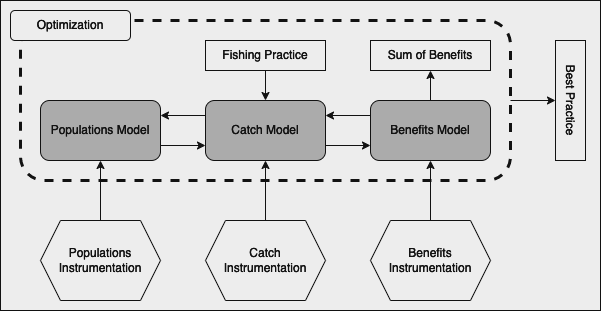
\includegraphics[width=\linewidth]{drawings/high_level_models.png}
  \caption{Models}
  \label{fig:high_level_models}
\end{figure}
\newline
\rule{\textwidth}{0.5pt} 
\vspace{5pt}

The first thing we need is a series of models that will allow us to... well... model how changing fishing practice will effect our overall benefit. These models divide into, broadly speak, three different categories. 
\newline

The benefits model is how we derive, from a specific situation, what the expected long term benefit would be. For example if the \textit{only} benefit is economic first sale benefit based on weight then the relationship between weight and cost would be one aspect of our model. This could then be applied to the expected catch each year (structured by weight of course) to then produce an expected value of the fishery year over year which could then be integrated to give us the long term benefit. In general however benefits models are far more complicated than this as, as we've already mentioned, there's a lot more to benefit that just value per weight class.
\newline

The second model we need is the population model. This describes how the populations in question change in response to the environment around them (which can include the fishers). A simple example would be a model that predicts the amount of recruitment (new fish babies) to the population as a function of the current population along with a model of how quickly the fish die off from natural mortality as the years go by. These two then allow us to predict how the population will change over time. However these models can get far more complex than just this (and most often do). 
\newline

In the middle of these two models we need a catch model. This is the model that describes how our choices in managing the fishery effect the underlying populations. Often times this model is as simple as a relationship between fishing effort and fishing mortality with some notion of gear selectivity included (gear selectivity being the fact that a specific kind of gear will typically catch a particular kind of age or weight of fish). Without this model there's no way to connect our benefit model to the population model. It's also the model that takes the parameters of fishery action that we're ultimately using as the knobs to tune to optimize our overall sustained benefit to society. 
\newpage

\noindent \rule{\textwidth}{0.5pt} 
\begin{figure}[h!] 
  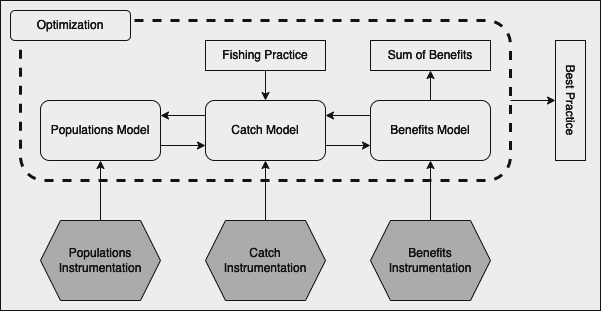
\includegraphics[width=\linewidth]{drawings/high_level_instrumentation.png}
  \caption{Instrumentation}
  \label{fig:high_level_instrumentation}
\end{figure}
\newline
\rule{\textwidth}{0.5pt} 
\vspace{5pt}

We've been talking about models quite flippantly so far. But all models are approximations of reality that need to be fit. What does fitting mean? Let's take a super simple example. You know gravity, the thing holding you to the ground right now (unless you're reading this in space, in which case I'm very jealous)? Well while you may take gravity for granted, in high school you learned about a specific model for it - Newton's theory of gravitation. As we've since learned thanks to Einstein, Newton's model breaks down in specific situations, but for the purposes of your being held to the ground the model does just fine. 
\newline

And it looks like this:
\newline

The model divides into three parts:

\begin{enumerate}
\item Input variables
\item Output variables
\item Parameters
\end{enumerate}

And here's the problem, in order to actually get anything out of this equation those parameters need to be given values. How to set those values? Well what we can do is take a whole bunch of measurements of both input and output values. We can then guess at a value for the parameters in the above equation. Then we can take our measured inputs, pass them through, get our predicted outputs, and evaluate how well we did predicting the outputs. Given what we find we can guess at another set of values for our parameters and repeat until we find the parameters that best fit our data. 
\newline

This being the real world, they're never going to fit absolutely perfectly (we'll get to what that means for fisheries later) but eventually we'll be able to find the closest fit and voila we have a gravitational constant!
\newline

This is how fitting works in general - you take real, measured data, and use that to choose the parameters of your model that best that data - the ground truth. And this means something very simple - each of our fisheries models needs ground truth data which in turn means that we need instrumentation for each of them in order to collect that ground truth data. 
\newline

\textbf{ADD DETAIL TO THIS SECTION}
\newpage

\noindent \rule{\textwidth}{0.5pt} 
\begin{figure}[h!] 
  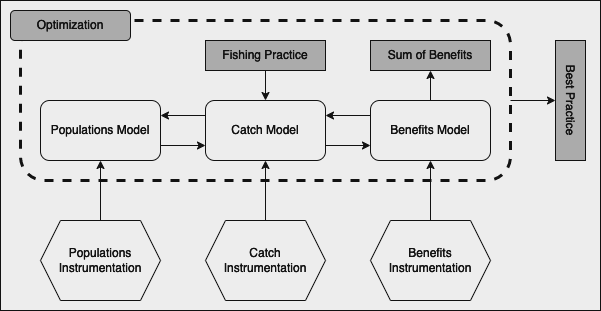
\includegraphics[width=\linewidth]{drawings/high_level_optimization.png}
  \caption{Optimization}
  \label{fig:high_level_optimization}
\end{figure}
\newline
\rule{\textwidth}{0.5pt} 
\vspace{5pt}

\textbf{ADD DETAIL TO THIS SECTION}
\newpage

\section{Risky Business}
\newpage

\section{Unparalleled Progress}
\newpage

\section{The Map}



\bibliographystyle{plain}
\bibliography{reference}
\end{document}